\begin{figure}[H]
    \begin{subfigure}[t]{0.33\textwidth}
        \caption{}
        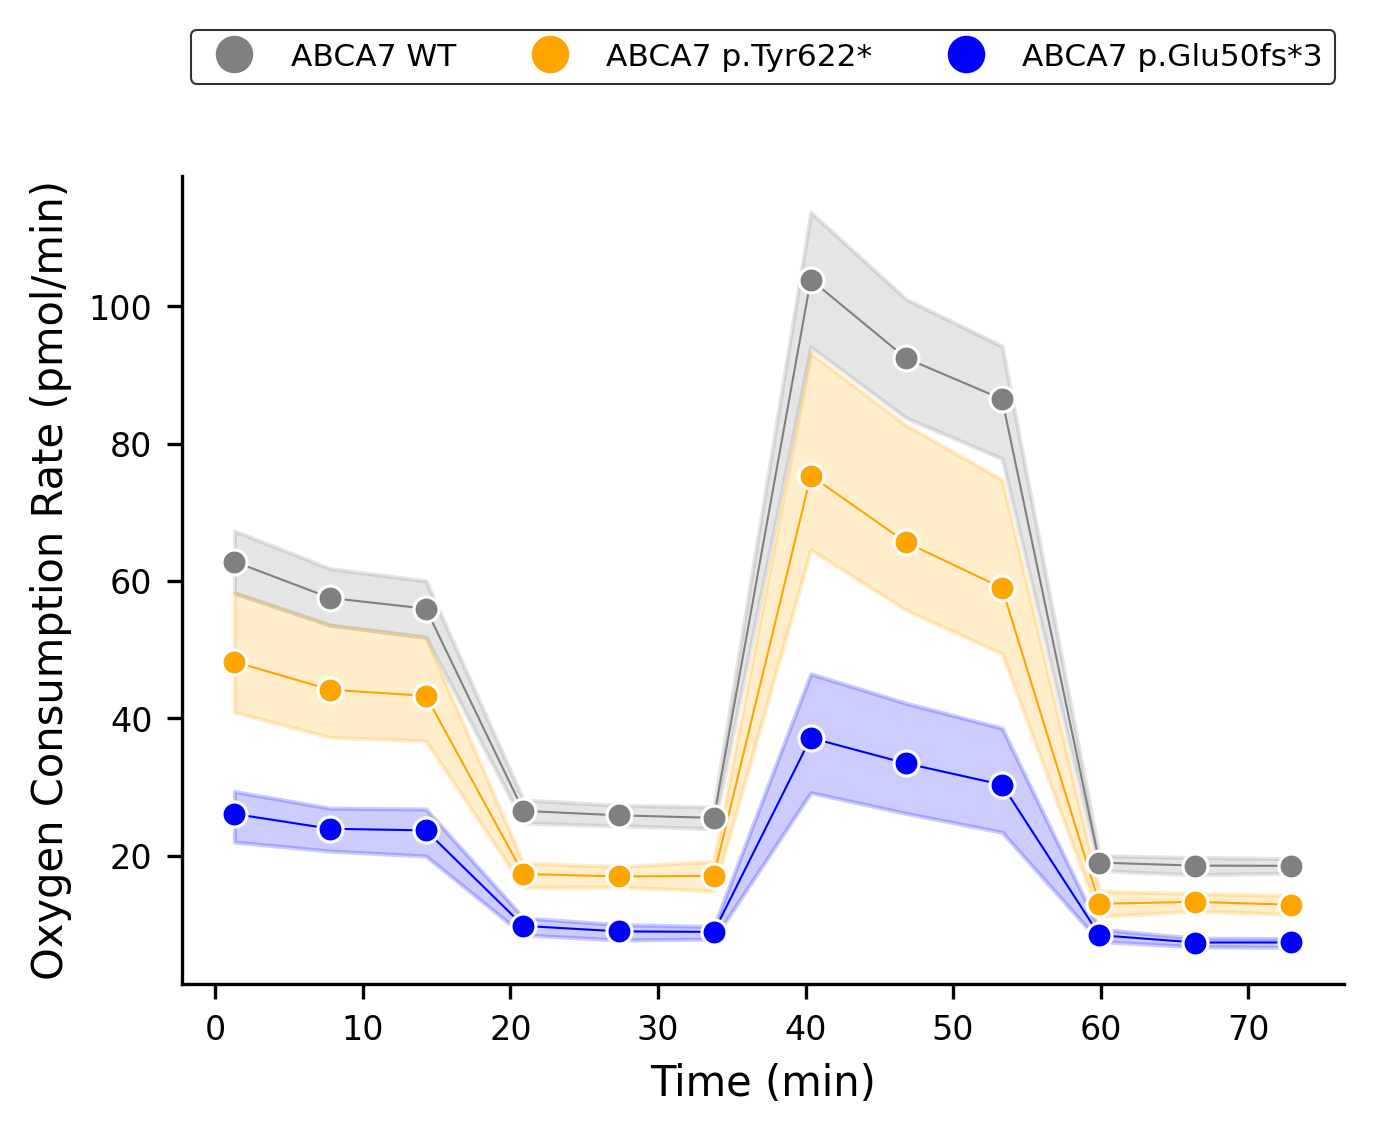
\includegraphics[width=\textwidth]{./extended_plots/rep_seahorse_curves_by_line.png}        
    \end{subfigure}
    \begin{subfigure}[t]{0.33\textwidth}
        \caption{}
        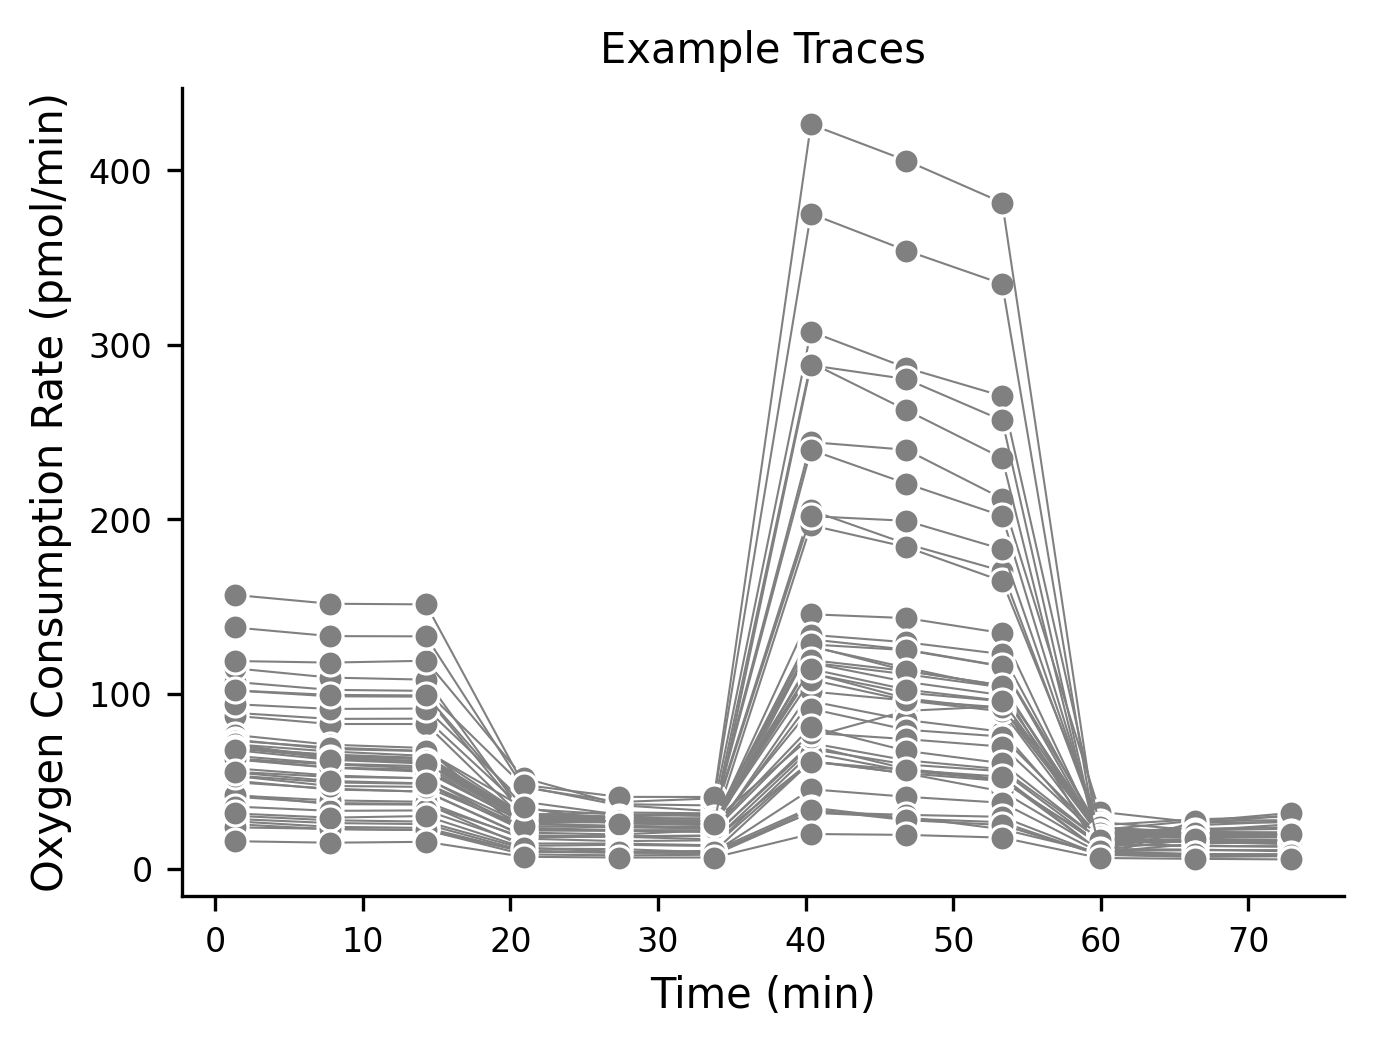
\includegraphics[width=\textwidth]{./extended_plots/rep_seahorse_curves_all.png}        
    \end{subfigure}   
    \begin{subfigure}[t]{0.33\textwidth}
        \caption{}
        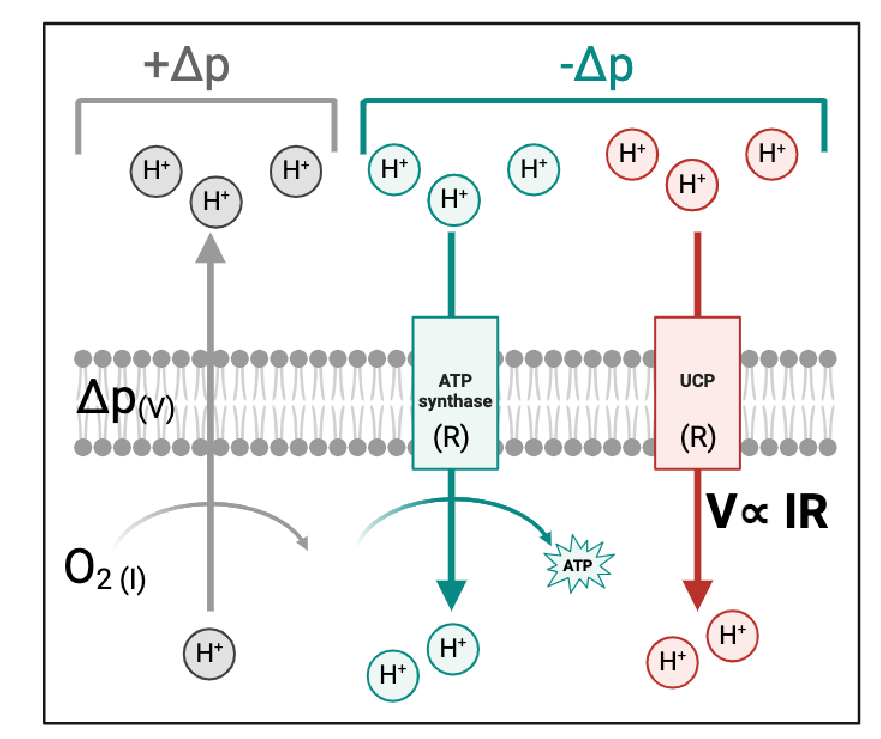
\includegraphics[width=\textwidth]{./main_plots/uncoupling_cartoon.png}        
    \end{subfigure}  
    \begin{subfigure}[t]{0.33\textwidth}
        \caption{}
        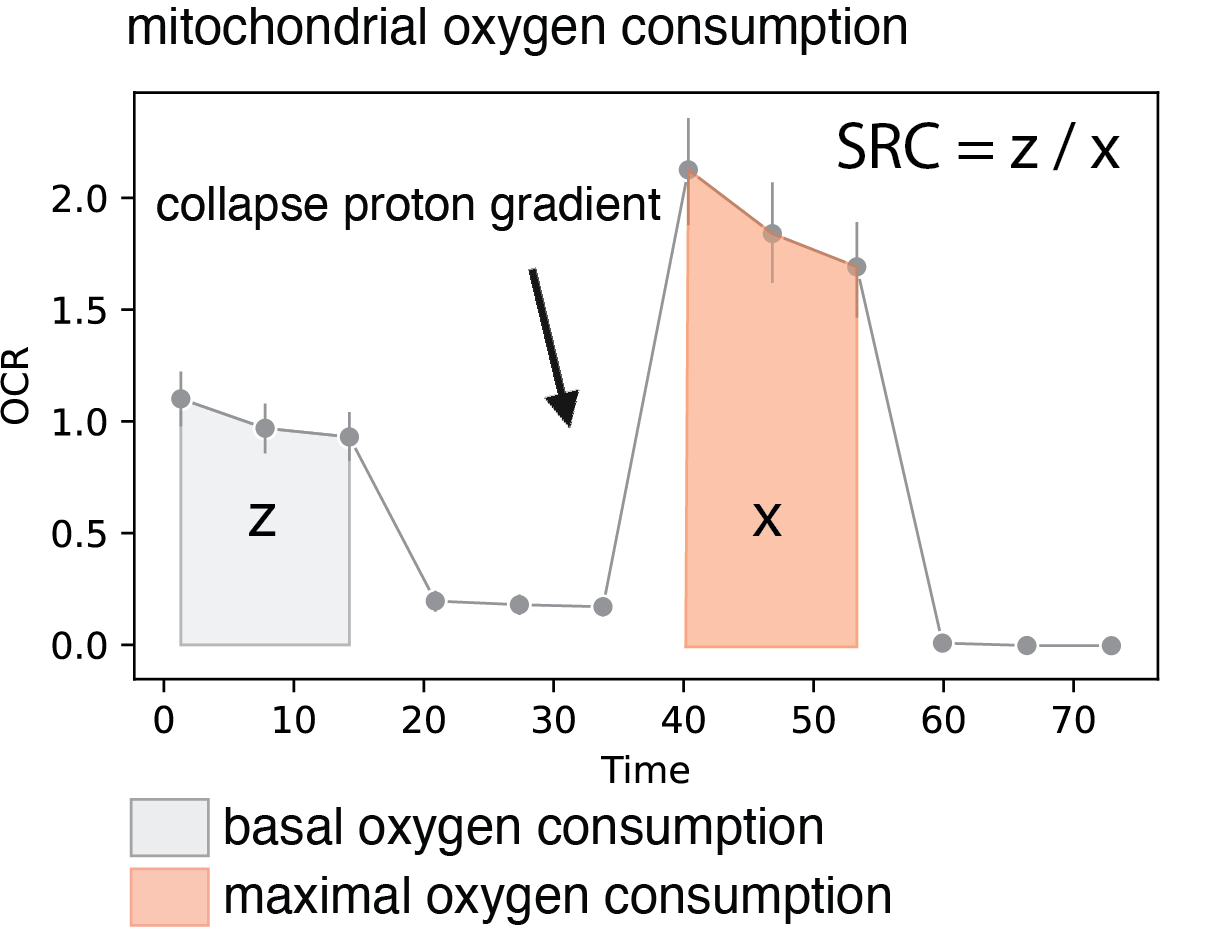
\includegraphics[width=\textwidth]{./extended_plots/src_cartoon.png}        
    \end{subfigure} 
    \begin{subfigure}[t]{0.33\textwidth}
        \caption{}
        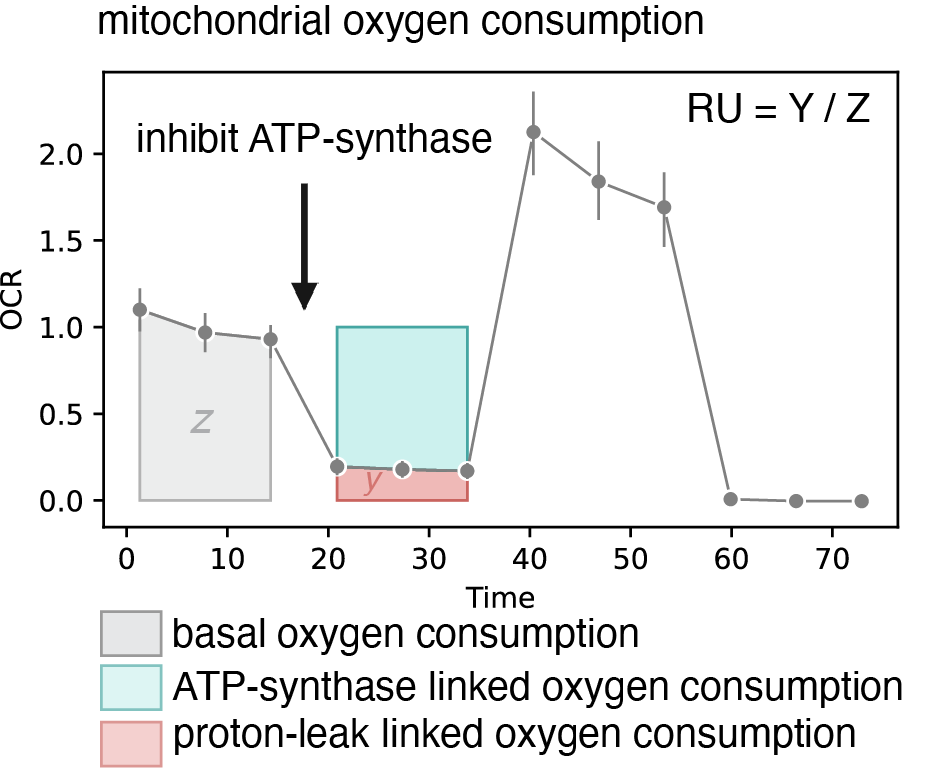
\includegraphics[width=\textwidth]{./main_plots/seahorse_cartoon.png}        
    \end{subfigure}  
    \begin{subfigure}[t]{0.25\textwidth}
        \caption{}
        \includegraphics[width=\textwidth]{./extended_plots/SRC.png}        
    \end{subfigure} 
    \begin{subfigure}[t]{0.25\textwidth}
        \caption{}
        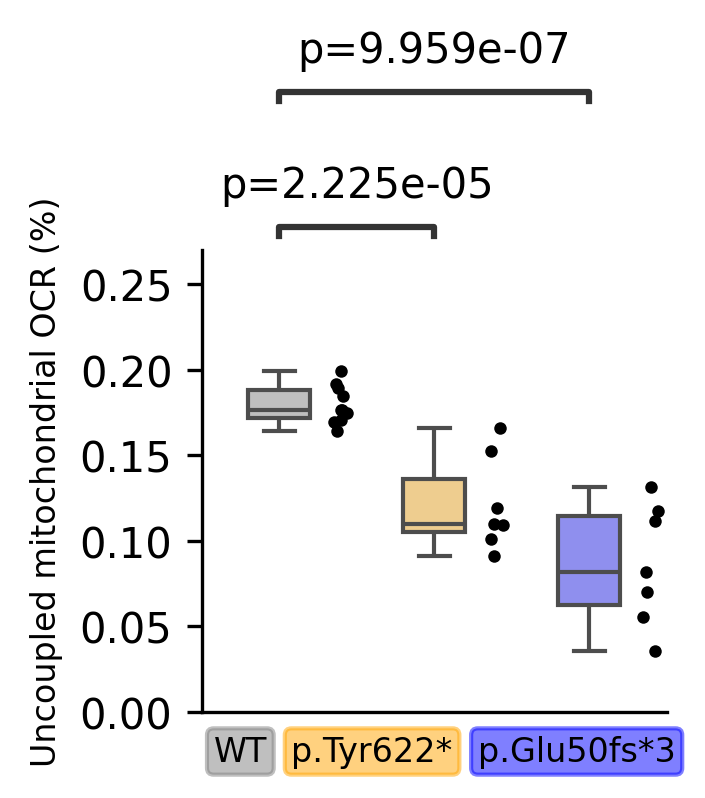
\includegraphics[width=\textwidth]{./extended_plots/uncoupling_quantification_batch1.png}        
    \end{subfigure} 
    \hspace{0.1\textwidth}
    \begin{subfigure}[t]{0.25\textwidth}
        \caption{}
        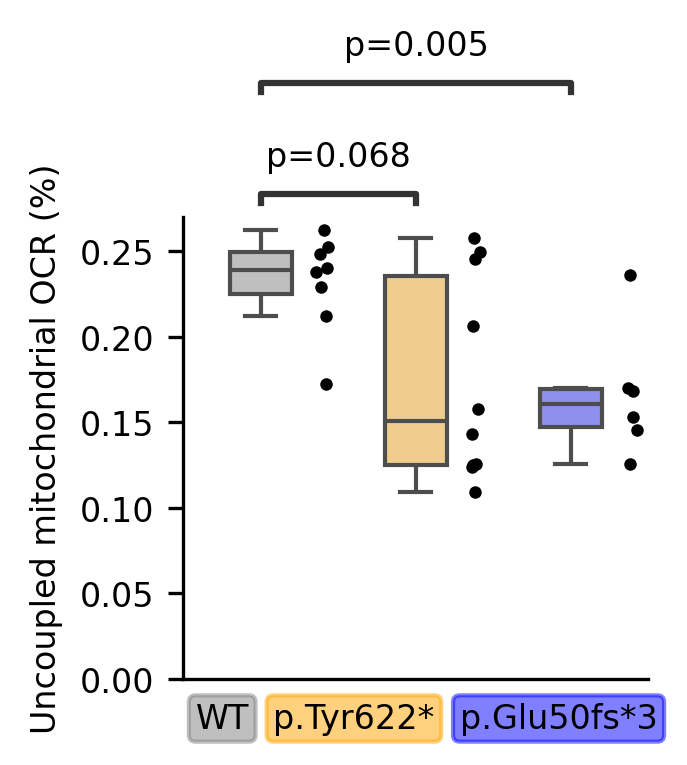
\includegraphics[width=\textwidth]{./extended_plots/uncoupling_quantification_batch2.png}        
    \end{subfigure} 
    \begin{subfigure}[t]{0.25\textwidth}
        \caption{}
        \includegraphics[width=\textwidth]{./extended_plots/UCP_levels.png}        
    \end{subfigure} 
    \caption{
         \textbf{Analysis of Oxygen Consumption Rates in ABCA7 LoF vs. Control iNs.}\\
     }
     \label{fig:oxygen_consumption_rates_iPSC_neurons}
 \end{figure}
 \begin{itemize}
    \item[\textbf{(A)}] Example oxygen consumption rate (OCR) curves from Batch 1 of the two differentiation batches used for analysis in Figure~\ref{fig:main_mitochondrial}G. The line plot indicates the per-condition mean estimator, and the error bars indicate the 95\% confidence interval. 
    \item[\textbf{(B)}] Representative per-well traces from (A). 
    \item[\textbf{(C)}] Schematic indicating the relationship between oxygen consumption as a measure of proton current (I), which sustains the proton motive force (voltage, V). Regulation of ATP synthase and uncoupling protein (UCP) activity modifies resistance (R) and depletes the proton motive force.
    \item[\textbf{(D)}] Schematic indicating measurement of maximal and basal oxygen consumption to compute SRC.
    \item[\textbf{(E)}] Schematic indicating measurement of uncoupled oxygen consumption.
    \item[\textbf{(F)}] SRC computed for WT, ABCA7 p.Glu50fs*3, and ABCA7 p.Tyr622* iNs. P-values computed by independent sample t-test. $N$ wells = 18 (WT), 17 (p.Tyr622*), 13 (p.Glu50fs*3) across two independent differentiation batches and Seahorse experiments. 
    \item[\textbf{(G, H)}] Relative uncoupling measured for two independent iN differentiation batches and separate Seahorse experiments shown combined in Figure~\ref{fig:main_mitochondrial}G. P-values computed by independent sample t-test. Batch 1 (left); $N$ wells = 10 (WT), 7 (p.Tyr622*), 7 (p.Glu50fs*3). Batch 2 (right); $N$ wells = 8 (WT), 10 (p.Tyr622*), 6 (p.Glu50fs*3) shown per differentiation batch.
    \item[\textbf{(I)}] UCP2 mRNA levels. 
 \end{itemize}